\documentclass{article}
\usepackage[%
    left=0.5in,%
    right=0.5in,%
    top=0.5in,%
    bottom=0.5in,%
]{geometry}%
\usepackage{minitoc}
\usepackage{multicol}
\usepackage{graphicx}
\graphicspath{ {./} }

\begin{document}
\section{Threads}

\begin{flushleft}
In computer science, a thread of execution is the smallest sequence of programmed instructions that can be managed independently by a scheduler, which is typically a part of the operating systems. (An independent set of values for the processor registers (for a single core)).
\end{flushleft}

\subsection{Theads from an OS perspective}
\begin{flushleft}
A proces consists of two \textbf{fundamental units}
\begin{itemize}
	\item \textbf{Resources}: all related resources are grouped together:
	\begin{itemize}
		\item A logical addres space containing the process image (program, data, heap stack)
		\item Files, I/O devices, I/O channels
	\end{itemize}
	\item \textbf{Execution trace}, i.e, an entity that gets exceuted
\end{itemize}
A process can \textbf{share its resources} between \textbf{multiple execution traces}. Every thread has its own \textbf{execution context} (e.g program counter, stack, registers).\\
All threads have \textbf{access} to the process \textbf{shared resources}
\begin{itemize}
	\item E.g files, one thread opens a file, all threads on the same process can acess the file
	\item Global variables, memory, etc. Which is needed or synchronisation
\end{itemize}
Some CPUs (hyperthreaded ones) have direct \textbf{hardware support} for \textbf{multi-threading}. They can offer up to 8 hardware threads per core.
\end{flushleft}
\bigskip


\begin{multicols}{2}
Similar to processes, threads have:
\begin{itemize}
	\item \textbf{States} and \textbf{transitions} (new, running, blocked, ready, terminated)
	\item \textbf{A thread control block}
\end{itemize}
Threads incur \textbf{less overhead} to create/terminate/switch (address space remains the same for threads of the same process)
\smallskip
\begin{center}
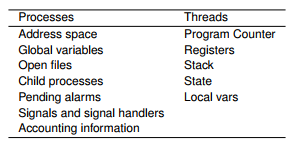
\includegraphics[scale=0.5]{Selection_007.png}
\end{center}
\end{multicols}

\begin{itemize}
	\item \textbf{Inter-thread communication} is easier/faster than \textbf{interprocess} communication (threads share memory by default)
	\item \textbf{No protection boundaries} are required in the address space. Threads are cooperating, belong to the same user, and have a common goal)
	\item \textbf{Synchronisation} has to be considered carfully
\end{itemize}

\subsection{Why use threads}
\begin{flushleft}
Multiple \textbf{related activites} apply to the \textbf{same resources}, these resources should be accessible/shared\\
Processes will often contain multiple \textbf{blocking tasks}
\begin{itemize}
	\item I/O operations (thread blocks, \textbf{interrupt} marks completion)
	\item Memory access: pages faults are result in blocking
\end{itemize}
Such activities should be carried out in \textbf{parallel/concurrently}. \textbf{Application examples}: webservers, make program, spreadsheets, word processors, processing large data volumes
\end{flushleft}

\pagebreak
\subsection{Thread types}
\begin{flushleft}
\begin{itemize}
	\item \textbf{User thread N:1}: To make threads \textbf{cheap and fast}, they need to be implemented at \textbf{user level}. User-Level threads are managed entirely by the \textbf{run-time system} (user-level library).The kernel knows nothing about user-level threads and manages them as if they were single-threaded processes.User-Level threads are \textbf{small and fast}, each thread is represented by a PC, register,stack, and small thread control block.
	\begin{itemize}
		\item \textbf{Advantages}
		\begin{itemize}
			\item A user-level threads package can be implemented on an Operating System that does not support threads.
			\item User-level threads do not require modification to operating system
			\item \textbf{Simple Representation}: Each thread is represented simply by a PC, registers, stack and a small control block, all stored in the user process address space.
			\item \textbf{Simple Management}: This simply means that creating a thread, switching between threads and synchronization between threads can all be done without intervention of the kernel.
			\item \textbf{Fast and Efficient}:  Thread switching is not much more expensive than a procedure call.
		\end{itemize}
		\item \textbf{Disadvantages}
		\begin{itemize}
			\item User-Level threads are invisible to the OS they are not well integrated with the OS. As a result, Os can make poor decisions like scheduling a process with idle threads, blocking a process whose thread initiated an I/O even though the process has other threads that can run and unscheduling a process with a thread holding a lock.
			\item Lack of coordination between threads and operating system kernel. Therefore, process as whole gets \textbf{one time slice} irrespect of whether process has one thread or 1000 threads within.
			\item User-level threads requires non-blocking systems call i.e., a multithreaded kernel. Otherwise, entire process will blocked in the kernel, even if there are runable threads left in the processes. For example, if one thread causes a page fault, the process blocks.
		\end{itemize}
	\end{itemize}
	\item \textbf{Kernel thread 1:1}: In this method, the kernel \textbf{knows} about and \textbf{manages} the threads. \textbf{No runtime system is needed} in this case. Instead of thread table in each process, the kernel has a thread table that keeps track of all threads in the system. Kernel-Level threads \textbf{make concurrency much cheaper} than process because, much less state to allocate and initialize.
	\begin{itemize}
		\item \textbf{Advantages}
		\begin{itemize}
			\item Because kernel has full knowledge of all threads, Scheduler may decide to give more time to a process having large number of threads than process having small number of threads.
			\item Kernel-level threads are especially good for applications that frequently block.
		\end{itemize}
	\end{itemize}
	\begin{itemize}
		\item \textbf{Disadvantages}
		\begin{itemize}
			\item The kernel-level threads are \textbf{slow and inefficient}. For instance, threads operations are hundreds of times slower than that of user-level threads.
			\item Since kernel must manage and schedule threads as well as processes. It require a full thread control block (TCB) for each thread to \textbf{maintain information} about threads. As a result there is significant \textbf{overhead} and increased in kernel complexity.		
		\end{itemize}
	\end{itemize}
	\item \textbf{Hybrid implementation M:N} maps some \textit{M} number of application threads onto some \textit{N} number of kernel entities or "virtual processors".In general, \textit{M:N} threading systems are more \textbf{complex} to implement than either kernel or user threads, because changes to \textbf{both kernel and user-space code are required}. In the \textit{M:N} implementation, the threading library is responsible for \textbf{scheduling} user threads on the available schedulable entities; this makes context switching of threads very fast, as it avoids system calls.
	\begin{itemize}
		\item \textbf{Advantages}
		\begin{itemize}
			\item Can take advantage of multiple CPUs or multiple CPU cores. And if one task blocks, you can create another kernel thread to use the available CPU more efficiently.
			\item Less context switches, which increases performance (in the ideal case, where you have as many running threads as you have processors, you may have almost no context switches).
		\end{itemize}
	\end{itemize}
	\begin{itemize}
		\item \textbf{Disadvantages}
		\begin{itemize}
			\item Possibly bigger latency: if all the threads in the pool are busy and you add new short task, you may wait a long time before it starts executing.
		\end{itemize}	
	\end{itemize}
\end{itemize}
\end{flushleft}

\subsection{Comparison}
\begin{center}
  \makebox[\textwidth]{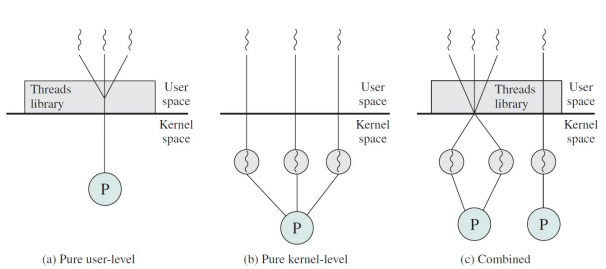
\includegraphics[scale=0.5]{Selection_002.png}}
\end{center}

\section{Libraries}
\subsection{Thread management}
\begin{flushleft}
Thread libraries provide an \textbf{API/interface for managing threads}. Can be implemented:
\begin{itemize}
	\item Entirely in \textbf{user space}
	\item Basedon \textbf{system calls}, i.e., rely on the kernel for thread implementations
\end{itemize}
Examples of thread APIs include \textbf{POSIX's PThreads}, Windows Threads and Java threads
\begin{itemize}
	\item The PThread specification can be implemented as user or kernel threads
\end{itemize}
\end{flushleft}

\subsection{POSIX Threads}
\begin{flushleft}
	POSIX threads are \textbf{specification} that \textbf{"anyone" can implement}. It definines a set of APIs (function calls, over 60) and what they do
\end{flushleft}
\end{document}
